\documentclass{exam}
\usepackage{../../mypackages}
\usepackage{../../macros}

%\usepackage{blindtext}

\SolutionEmphasis{\color{blue}}
\renewcommand{\solutiontitle}{\noindent}

\renewcommand{\arraystretch}{1.5} % Augmente l'espacement vertical entre les lignes du tableau
\newcolumntype{C}{>{\centering\arraybackslash}m{2cm}}

\SetLabelAlign{myright}{\hss\llap{$#1$}}
\newlist{where}{description}{1}
\setlist[where]{labelwidth=2cm,labelsep=1em,
                        leftmargin=!,align=myright,font=\normalfont}

\setlength{\parindent}{0pt}

\title{Interrogation N°2 - Sections}
\author{N. Bancel}
\date{9 Janvier 2024}

\begin{document}


\textbf{Collège Lycée Suger}
\hfill
\textbf{Mathématiques} \\

\textbf{Année 2024-2025}
\hfill
\textbf{1ères STD2A} \par

{\let\newpage\relax\maketitle}
%\maketitle


  \begin{center}
    \textbf{\textcolor{blue}{Durée du devoir : 30 minutes}} \par
    \vspace{1em}
    \textbf{\textcolor{red}{La calculatrice EST autorisée. Total des points : 20 points}} \par
    \vspace{1em}
  \end{center}
  
  \begin{tcolorbox}[colback=gray!10!white, colframe=gray, title=Note importante]
    Toutes les réponses doivent être justifiées : une réponse sans justification est considérée comme fausse. \par
  \end{tcolorbox}

\section*{Exercice 1 - Cours - 6 points}

\begin{questions}

  \question[3] Quelles sont les caractéristiques / propriétés de la perspective parallèle ? Dessiner un cube en perspective parallèle.

  \begin{solution}

    La perspective parallèle est une forme de perspective obéissant aux deux règles suivantes :
    \begin{compactitem}
        \item la représentation d'une droite restera une droite,
        \item le parallélisme sera conservé.
    \end{compactitem}
    
    La perspective parallèle peut être vue comme la projection sur un plan \(P\) suivant une direction donnée (\(d\)).
    

    Les propriétés de la perspective parallèle sont les suivante : 
    \begin{compactitem}
      \item L'image d'une droite étant une droite, la perspective parallèle « conserve » l'alignement.
      \item L'image de deux droites parallèles sont deux droites parallèles.
      \item L'image du milieu d'un segment est le milieu du segment image et plus généralement les rapports de longueurs sont conservés.
      \item Tout objet situé dans un plan parallèle au plan de projection a une image « en vraie grandeur ». Les angles et les distances sont alors conservés. Un objet parallèle au plan de projection est dit \textbf{frontal}.
  \end{compactitem}

  \begin{figure}[H]
    \centering
    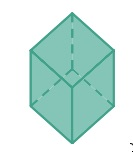
\includegraphics[width=0.5\linewidth]{img/interro_2_sections_01.jpg}
    \captionsetup{labelformat=empty}
    \caption{\label{} Cube en perspective parallèle}
  \end{figure}
  \end{solution}

\question[3] Quelles sont les caractéristiques / propriétés de la perspective cavalière ? Dessiner un cube en perspective cavalière.

\begin{solution}


La perspective cavalière est une perspective parallèle pour laquelle le plan de projection est un plan de face, c'est-à-dire un plan perpendiculaire au sol.  

Soit $(Ox)$ l'axe horizontal, parallèle au sol, et $(Oz)$ l'axe vertical, perpendiculaire au sol. En perspective cavalière :  
\begin{compactitem}
    \item l'angle entre ces deux axes reste de $90^\circ$,
    \item le rapport de réduction suivant ces deux axes est le même, ce qui signifie que les objets ne sont pas déformés suivant ces deux directions.
\end{compactitem}

L'axe $(Oy)$, perpendiculaire à $(Ox)$ et $(Oz)$, fait un angle arbitraire avec l'axe $(Ox)$. Le plus souvent, cet angle est de $45^\circ$ ou $30^\circ$. Le rapport de réduction est lui aussi arbitraire, mais il est le plus souvent fixé à 0,5 ou 0,7.


  \begin{figure}[H]
    \centering
    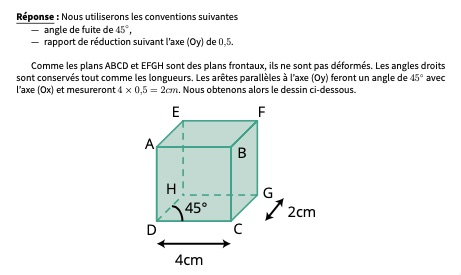
\includegraphics[width=0.5\linewidth]{img/interro_2_sections_02.jpg}
    \captionsetup{labelformat=empty}
    \caption{\label{} Cube en perspective cavalière}
  \end{figure}
  \end{solution}

\end{questions}


\section*{Exercice 2 - Dessin d'une section - 7 points}

\begin{questions}

\question[7]  Tracer la section du cube $ABCDEFGH$ par le plan $(IJK)$, en décrivant chacune des étapes de construction de celle-ci.

\begin{figure}[H]
  \centering
  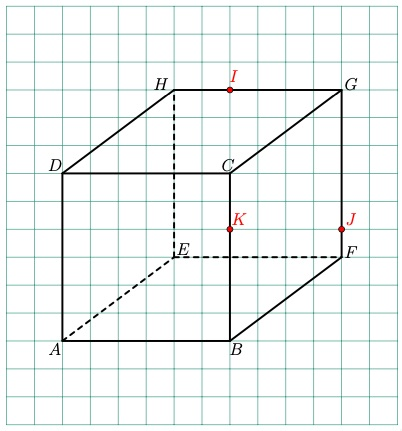
\includegraphics[width=0.8\linewidth]{img/interro_2_sections_03.jpg}
  \captionsetup{labelformat=empty}
  \caption{\label{}}
\end{figure}
\begin{solution}
  \begin{figure}[H]
    \centering
    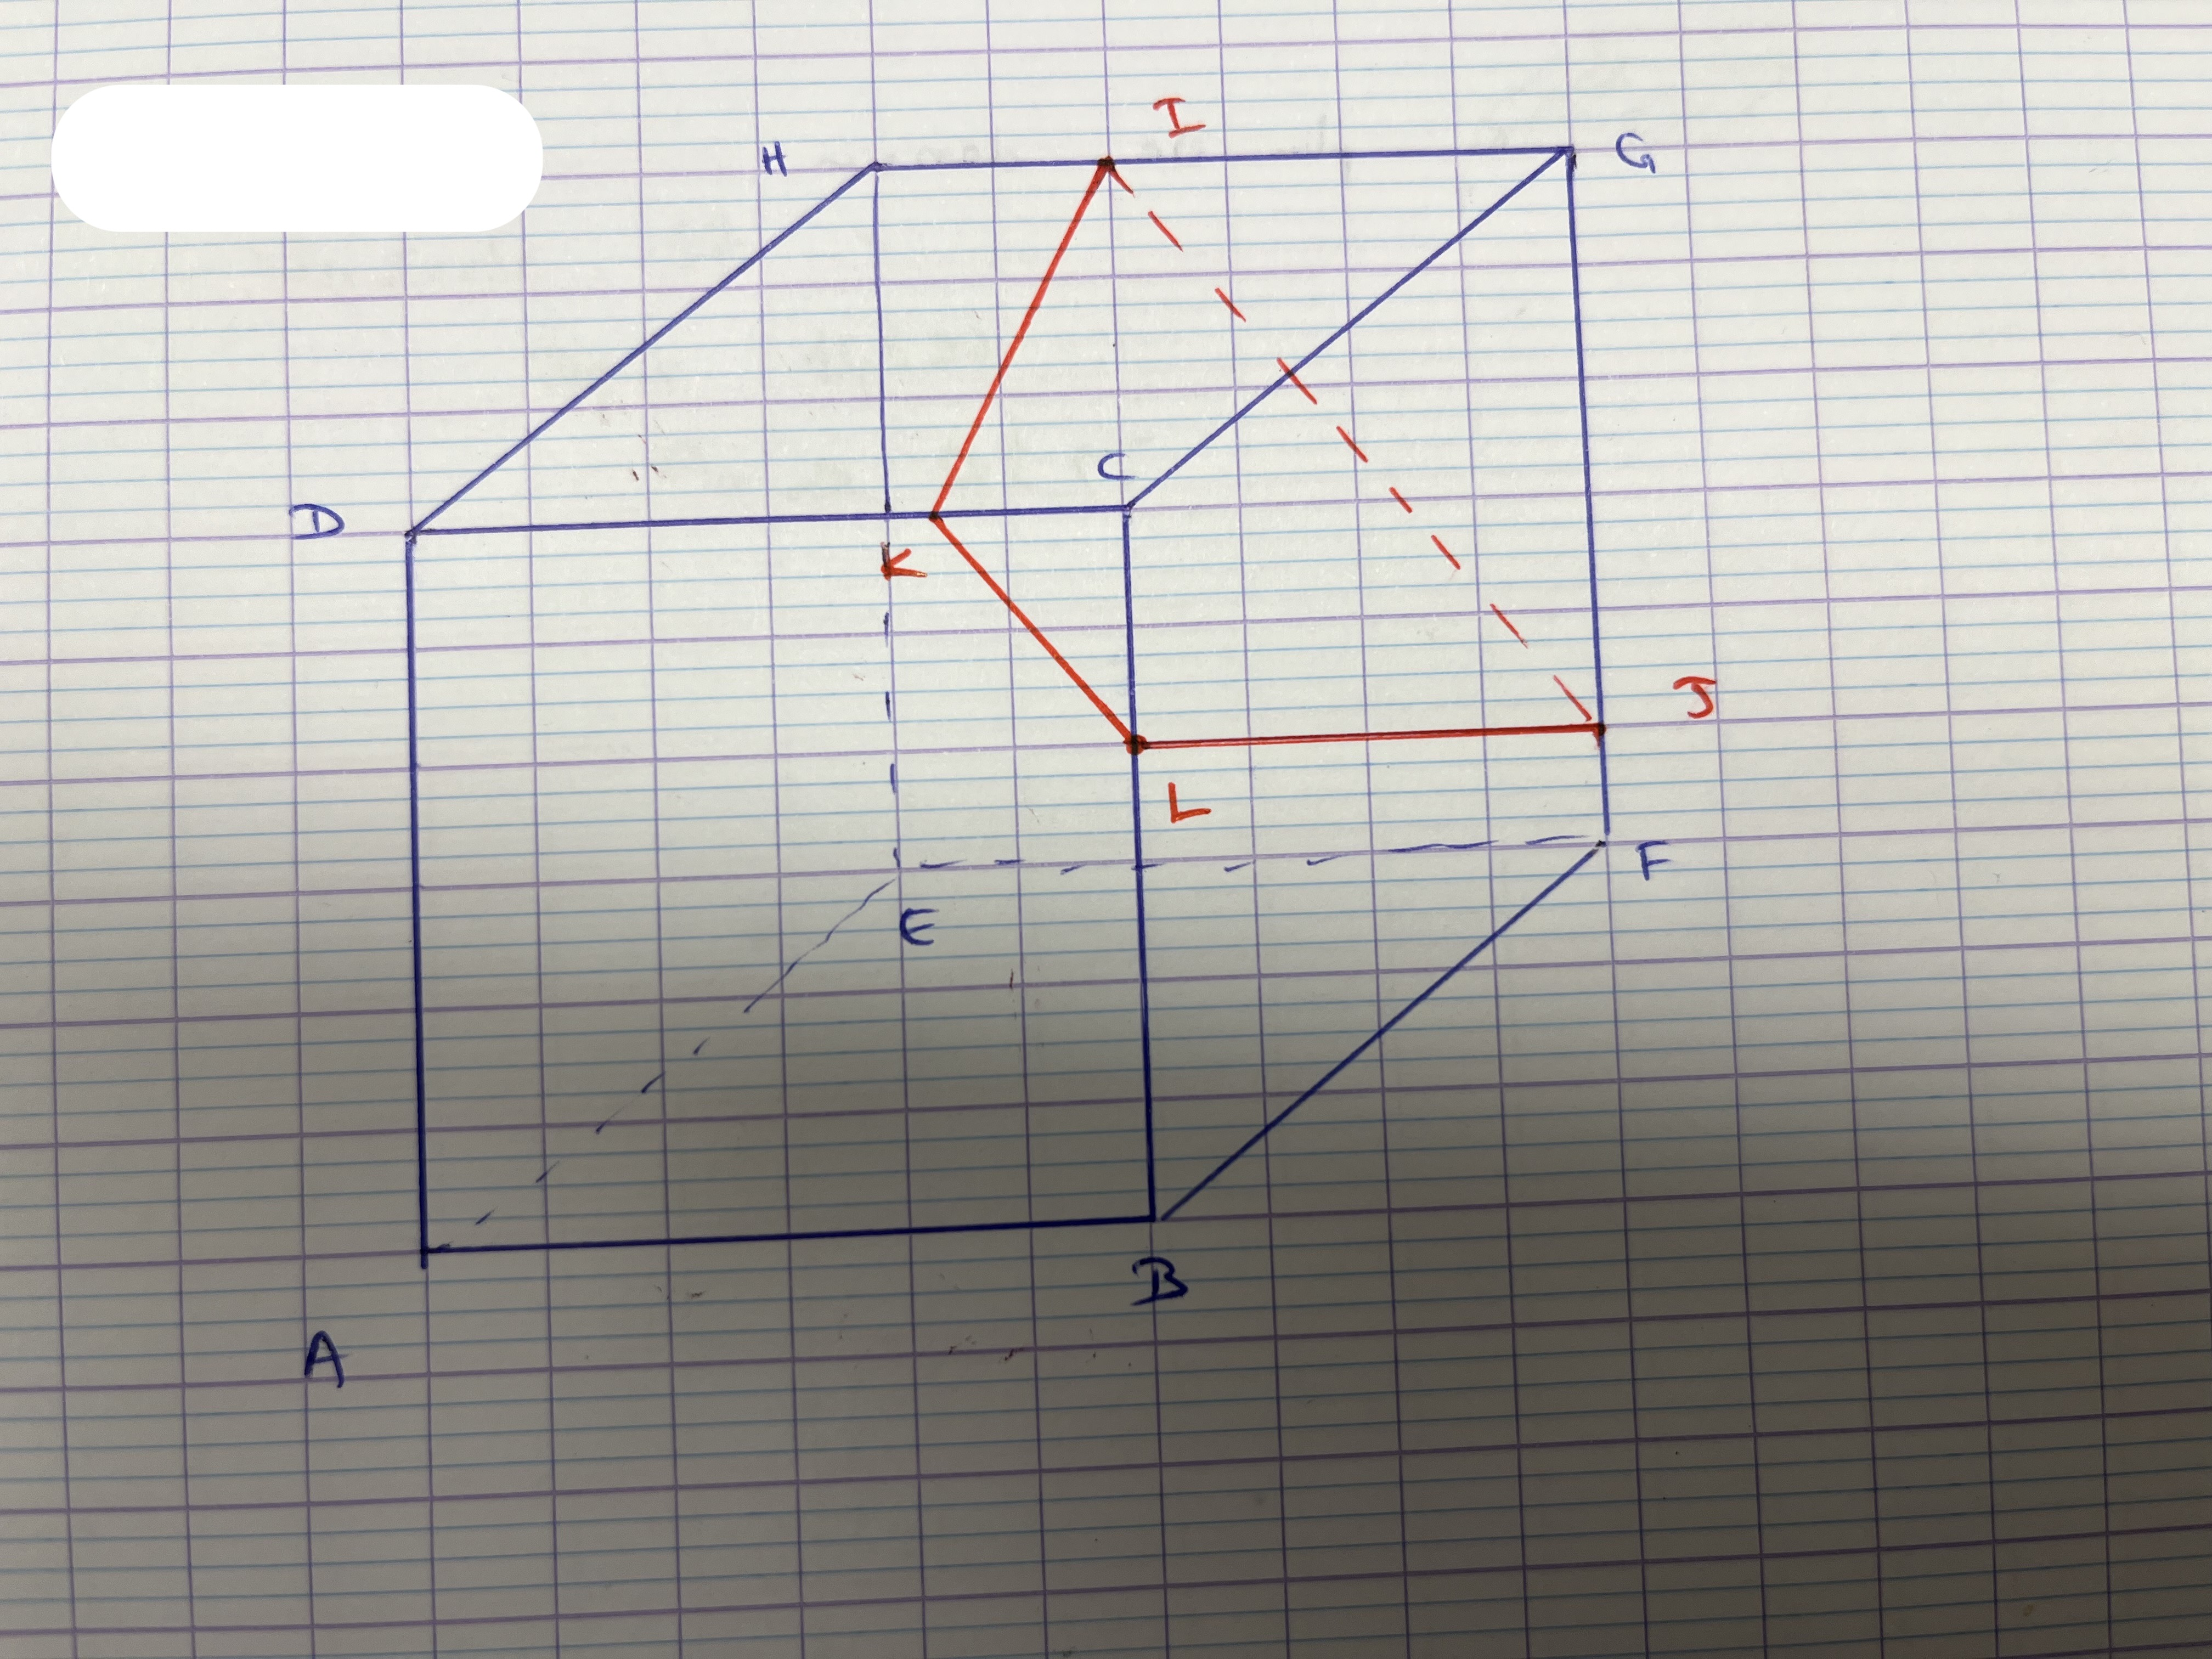
\includegraphics[width=0.8\linewidth]{img/interro_2_sections_05.jpeg}
    \captionsetup{labelformat=empty}
    \caption{\label{}}
  \end{figure}
\end{solution}
\end{questions}

\section*{Exercice 3 - Dessin d'une section - 7 points}

\begin{questions}

  \question[7]  Tracer la section du cube $ABCDEFGH$ par le plan $(IJK)$, en décrivant chacune des étapes de construction de celle-ci.
  
  \begin{figure}[H]
    \centering
    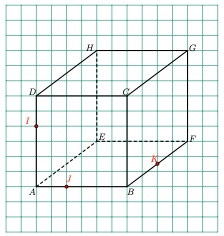
\includegraphics[width=0.8\linewidth]{img/interro_2_sections_04.jpg}
    \captionsetup{labelformat=empty}
    \caption{\label{}}
  \end{figure}
  \begin{solution}
    \begin{figure}[H]
      \centering
      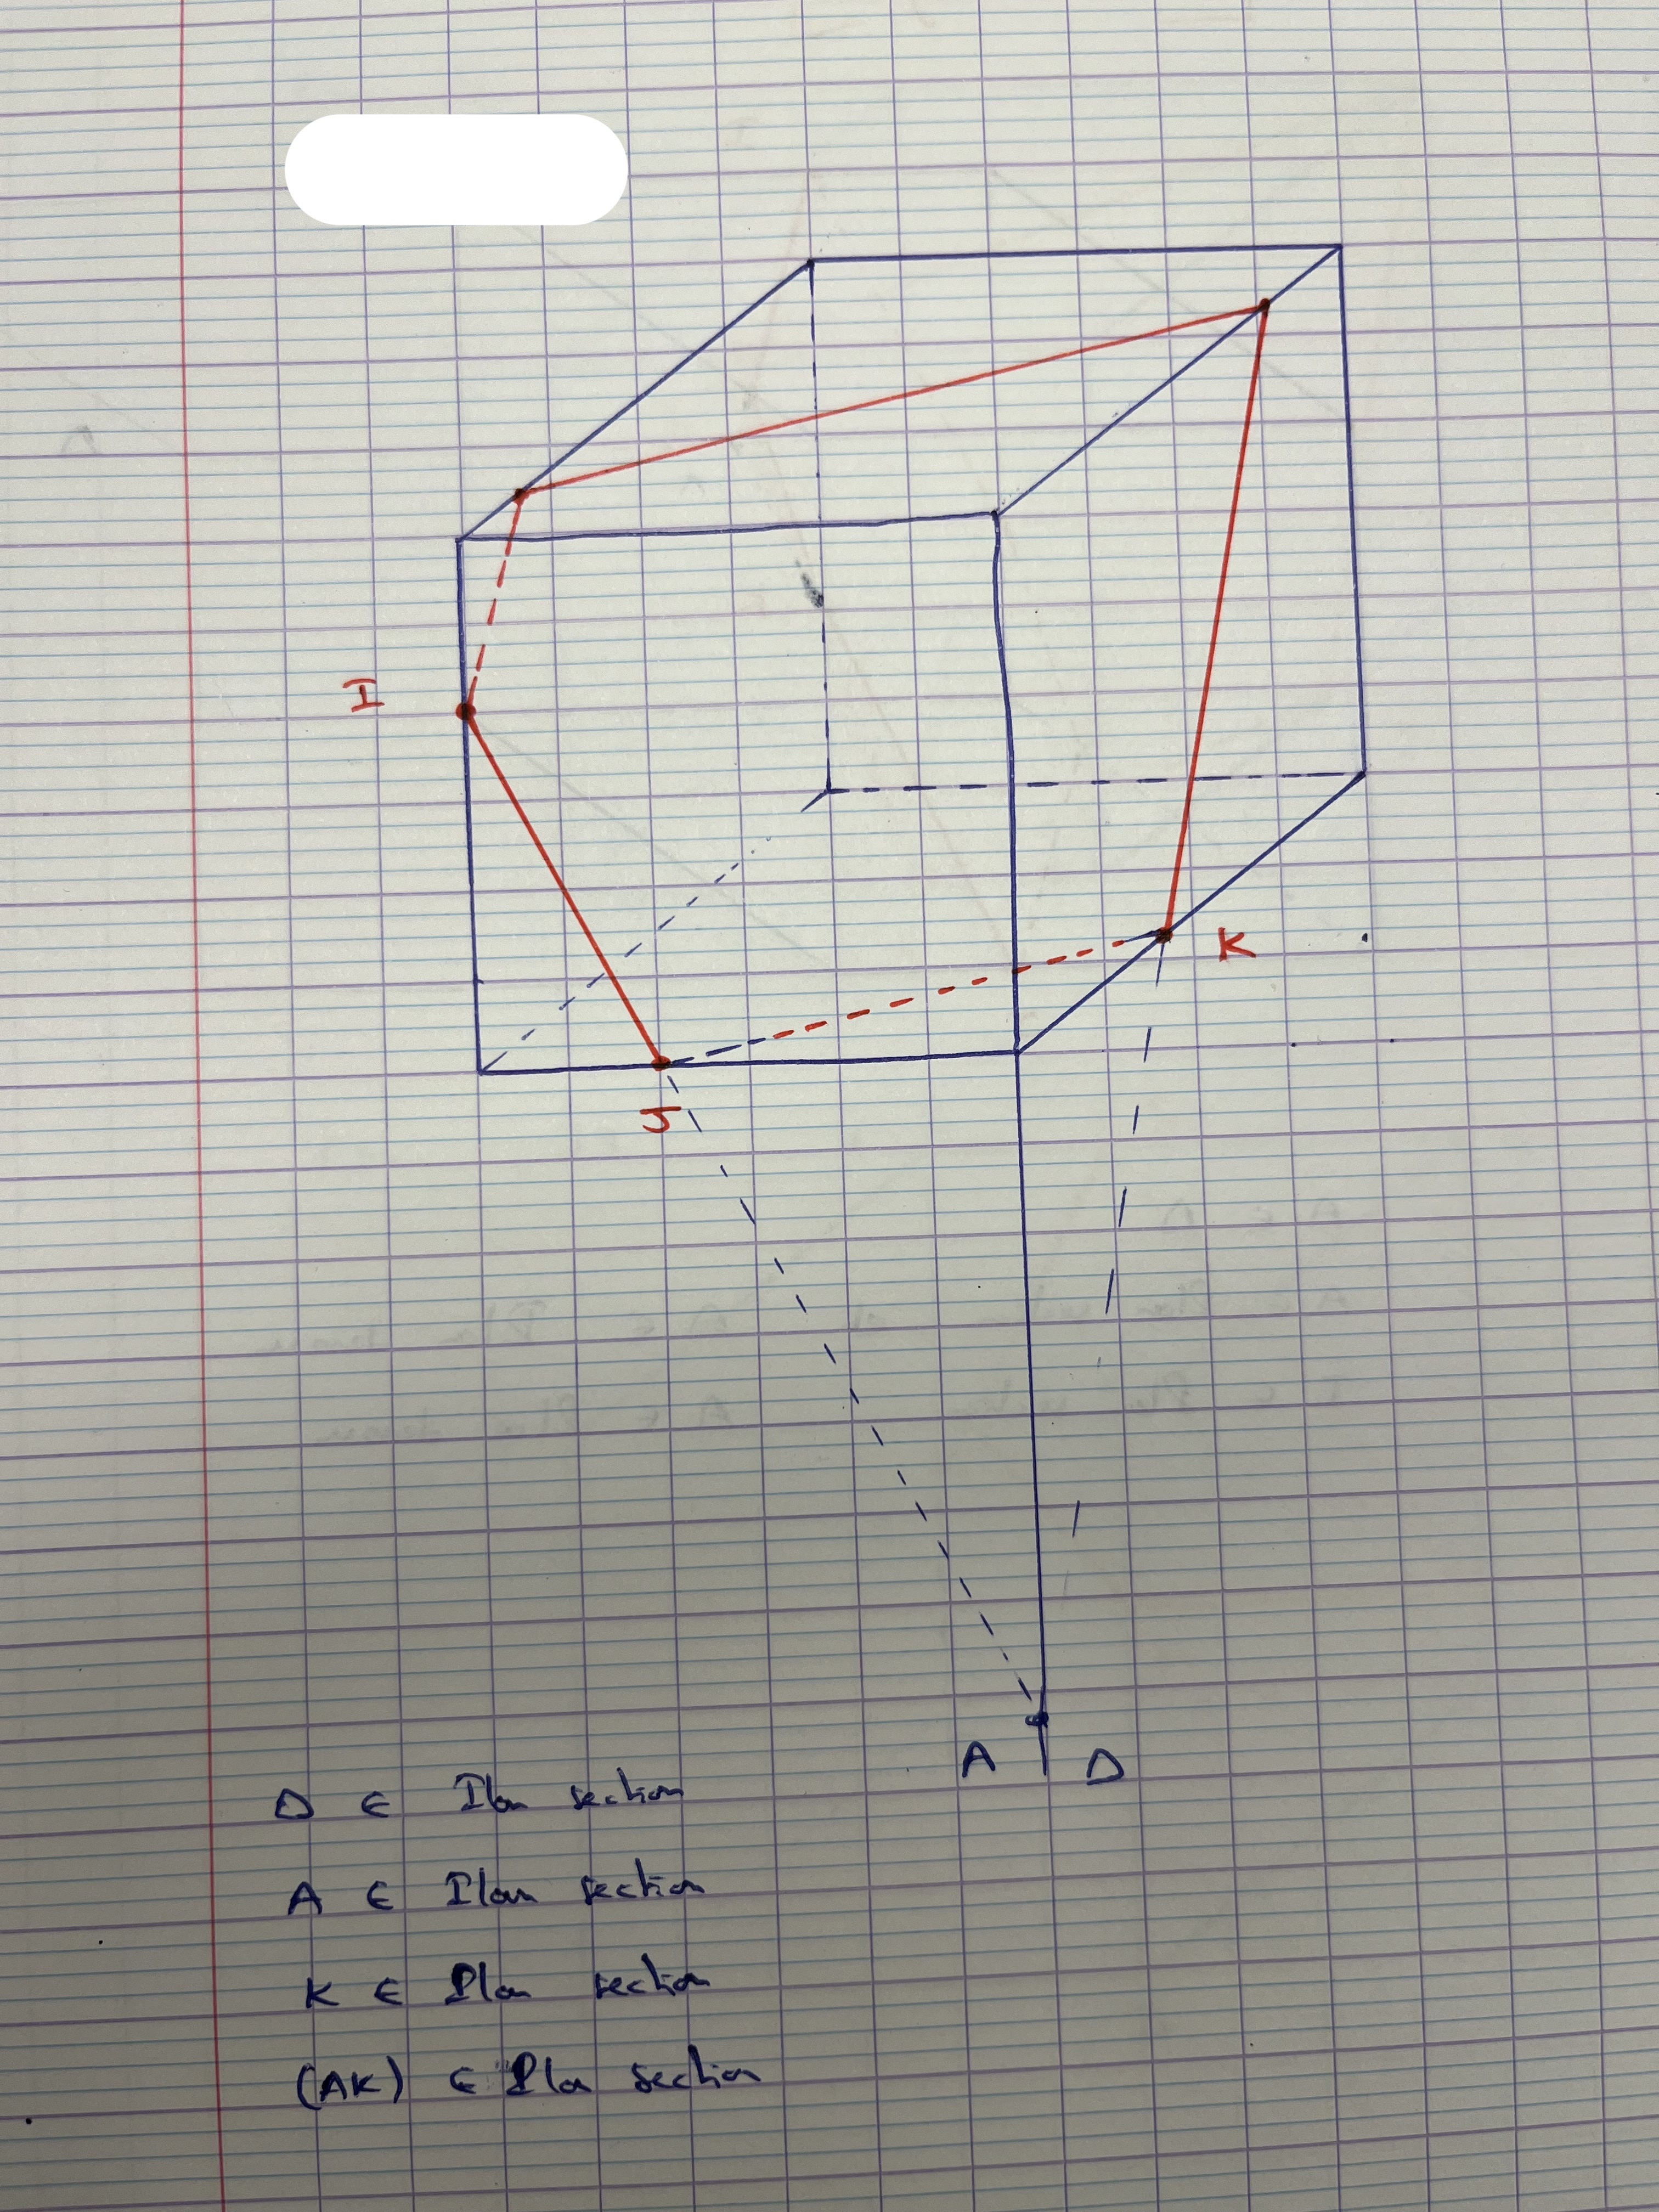
\includegraphics[width=0.8\linewidth]{img/interro_2_sections_06.jpeg}
      \captionsetup{labelformat=empty}
      \caption{\label{}}
    \end{figure}
  \end{solution}

\end{questions}



\end{document}
